\documentclass[algorithmlist, figurelist,tablelist, nomlist,masters]{seuthesix}


\begin{document}
\categorynumber{000} % 分类采用《中国图书资料分类法》
\UDC{000}            %《国际十进分类法UDC》的类号
\secretlevel{公开}    %学位论文密级分为"公开"、"内部"、"秘密"和"机密"四种
\studentid{130623}   %学号要完整,前面的零不能省略。
\title{灵犀一指心法}{灵犀一指}{The theory of powerful fingers}{powerful fingers}
\author{陆小凤}{Phoenix Land, Jr.}
\advisor{夜帝}{教授}{King Night}{Prof.}
\coadvisor{楚留香}{副教授}{Perfume Tsu}{Associate Prof.} % 没有% 可以不填
 \degreetype{武学硕士}{Master of kung fu} % 详细学位名称
\major{内功}
\submajor{内功心法}
\defenddate{\today}
\authorizedate{\today}
\committeechair{夜帝}
\reviewer{张三丰}{黄药师}
\department{东南大学武学院}{School of kung fu}
\seuthesisthanks{本课题的研究获郭靖-黄蓉降龙基金、杨过-小龙女黯然销魂基金以及郭襄的倚天基金资助}
\makebigcover
\makecover
\begin{abstract}{武功,心法,内功,灵犀一指}
灵犀一指是一种非常厉害的武功。
\end{abstract}

\begin{englishabstract}{kung fu, theory, fundamental kung fu, powerful fingers}
 powerful fingers is a kind of powerful kung fu.
\end{englishabstract}

\setnomname{术语与符号约定}
\tableofcontents
\listofothers

\mainmatter

\chapter{绪论}
\section{研究背景}
循证医学(Evidence-based medicine,EBM)[1],其核心思想是医生在做医疗决策的时候应遵循现有的最好的临床研究证据,并结合个人的临床经验,制定出适合病人的治疗措施。EBM是现代医学成熟稳健、睿智理性的核心。EBM从精心设计和精心实施的研究提供的证据中获得临床决策支持,这些证据包括问题分析、系统综述(Systematic Reviews, SR)和随机对照实验(Randomized Controlled Trials,RCTs)等。在实际应用中,证据的收集通常依赖医师手工搜索和分析文献。但医学文献种类旁多,更新迭代快,即便是一个细分的领域也有很多文献,例如PubMed医学文献数据库提供的文献已经达到了千万级别。除此之外,医学文献常以非结构文本形式的刊物存在,医师需要仔细阅读,避免遗漏证据的任何细节。

近些年医学文献的爆发式增长使得医师为了掌握某一个课题的最新医学研究成果不得不花费大量时间和精力阅读各种期刊文献。为了促进EBM在临床中的应用,一个非常关键的研究领域便是医学证据的规范化,使得证据可以被机器理解和处理。因此,PICO框架[2]被广泛应用于EBM。PICO是一种将信息规范化的方式,它将问题分为四个部分:问题/人口(Population/Problem)、干预(Intervention)、对照实验(Comparison)和结果(Outcome),有关临床医学证据的医学文献中重要的信息描述往往围绕PICO框架来展开。对医学文献中的PICO元素进行自动提取能减轻临床医生在证据收集和理解上的负担,大幅度提高循证医学的效率。
另一方面,医学文本挖掘方法近几年得到了长足的进步[3-8],可以从电子病例中挖掘病人信息、根据某项疾病统计患者的年龄分布,以及根据每一项症状和检查指标推荐可能有效的药品等。为了加速循证医学的实践,帮助医师快速获得文献关键证据,基于PICO的医学文献摘要研究也越来越多。任务流程可以理解为从医学文献的摘要或全文中抽取PICO相关的句子作为医学证据摘要。但大部分方法通常仅利用了医学文献的文本特征,如文章关键词、词频、句子长度等,忽略了医学知识的利用。知识图谱[9] (Knowledge Graph)近几年发展迅速,其作为一种语义网络拥有极强的表征能力和建模的灵活性。它可以对现实世界中的实体、概念、属性以及它们之间的关系进行建模。知识图谱可以看作是一种特殊的图数据结构,含有大量的结构化信息。知识图谱为基于知识的任务带来了极大的价值,丰富的特征能够有效提升任务结果,利用方式一般分为两种:一种是利用图表示学习技术(又叫网络表示学习)将知识图中的结点或者关系嵌入到一个低维空间中再加以利用,不同的方法可以捕捉不同的信息,比如图的属性信息[10-13]、上下文信息[14]、结构信息[15]和连接信息[16]等。代表技术有基于随机游走[17,18]的方法、基于矩阵分解[19-21]的方法等。另一种是随着图神经网络[23-25]的兴起,将神经网络直接作用于图结构数据的利用方式开始流行起来。与先前的图表示学习模型不同,图神经网络背后的关键思想是通过神经网络聚合节点邻居的信息特征来丰富节点表示。

目前存在大量的医学知识图谱,包括UMLS、DrugBank等。医学概念(Medical Concept)即医学知识图谱中的实体,如疾病、药物、基因等。医学知识图谱中包含医学概念丰富的实体属性和连接关系等信息,这些医学知识可以为医学文献挖掘提供高质量的结构化特征,提高医学文献摘要结果质量,形成知识驱动的医学文献摘要。经过调研,基于知识图谱的医学文献摘要主要存在以下问题:(1)医学知识的多源性:基于PICO的医学文献摘要结果涉及领域广泛,目前的方法缺乏对医学知识图谱的利用,更缺乏对多领域、多知识图谱的挖掘。比如蛋白质知识图谱、基因知识图谱、药物知识图谱等,它们涵盖了医学知识的一个领域,但知识之间又有关联。如果能将这些知识医学图谱结合起来,无疑能够对文献摘要任务起到巨大的提升作用。在摘要过程中为了充分利用这些不同领域的知识,需要进行跨知识图谱的医学表示学习,将丰富的医学知识刻画为可计算的低维向量;(2)医学知识的异构性:医学知识中涉及大量的医学概念,而不同的医学概念除了存在复杂的相互关系之外,还存在文本描述、图片描述、值描述等异构(Homogeneous)属性。基于PICO的医学文献摘要结果中常包含很多病人、疾病、药物等对象的多种属性信息,比如疾病的描述、药物描述、药物状态和剂量等。但目前相关研究对属性的利用方式还比较单一,使得最终医学实体嵌入对网络信息的存储有限。因此在医学表示学习的过程中需要考虑医学知识的异构特征,提出基于异构特征的医学表示学习方法,精确刻画医学知识之间的相关性和差异性。深入挖掘和利用属性特征,使得医学实体蕴含更丰富的知识并应用于医学文献摘要,对于提升摘要质量具有重大意义。

针对以上问题,本文提出了基于知识图谱的医学文献摘要方法,将知识图谱进行表示学习后用于医学文献摘要任务。在医学表示学习的过程中充分考虑了医学知识的多源性和异构性,在将复杂的医学知识表征为可计算的低维向量时,不仅考虑了来自多个医学图谱的不同领域的医学知识,还刻画了医学知识的异构特征,实现了知识驱动的医学证据摘要。

综上所述,尝试利用多领域、多个医学知识图谱信息相互补充,并挖掘知识图谱实体的异构属性特征,将医学知识应用于提升医学文献质量,为临床决策提供支持,是值得研究的方向。这不仅有极大的科研价值,而且对询证医学领域的发展、减轻医师的工作负担等都有非常大的实际应用价值。



\section{国内外研究现状}
医学文献摘要领域不断有新的研究工作希望能够打破传统的文本驱动的方式[29],融入医学知识图谱中的结构化医学知识,从而提升医学文献摘要质量。在知识图谱现有的利用方式上,还是以网络表示学习为主流。将知识图谱看作同质图(Homogeneous Graph),实体或关系通过模型转变为低维空间向量,从而方便作为下游任务的输入。除此之外,近两年图神经网络迅猛发展,它能够编码更高维度的信息,方便扩展利用属性特征信息,对知识图谱的利用更加充分,针对特定任务取得了更好的结果。总的来说,本节的研究现状主要从网络表示学习、图神经网络和医学文献摘要抽取三个方面进行阐述。

\subsection{网络表示学习现状分析}

网络表示学习(也称为图表示学习),旨在将实体和关系映射到低维空间向量中,方便作为下游任务的输入,从而可以帮助我们更好地利用知识图谱中的知识。代表技术有基于随机游走[17-18]的方法、基于矩阵分解[22-24]的方法等。

基于随机游走的代表方法是DeepWalk[18],基本假设是如果节点在某条随机游走序列中同时出现,那么表征这些节点存在某种近似。针对网络中的每个节点进行随机游走,游走过程中就得到了一系列的有序节点序列,这些节点序列可以类比到自然语言文本处理中文章的句子,节点类比于句子中的单词,然后使用Skip-gram模型[30]训练得到节点的嵌入表示。

Node2Vec[17]是对DeepWalk的改进,主要的创新点在于改进了随机游走的策略,定义了两个参数p和q。超参数p控制了访问前一节点的概率,q控制访问节点的直接邻居的概率,在广度优先搜索和深度优先搜索中达到一个平衡,同时考虑到局部和宏观的信息,并且具有很高的适应性。

LINE[31]模型提出了一阶相似度和二阶相似度的概念,一阶相似度计算对象是直接相连的节点,二阶相似度计算对象通过其他中介节点相连的节点,即具有共享邻居节点的节点可能是相似的。LINE在概念上与Node2Vec和DeepWalk有关,因为它使用了概率解码器和损失函数,但它明确地分解了一阶和二阶相似度,而不是将它们组合成固定长度的随机游走序列。

矩阵分解的方法受到经典的降维技术的启发[32],主要有拉普拉斯特征映射、内积方法,其基本假设是结点之间的关系强度与结点向量点积结果成正比。不同方法主要区别是距离衡量函数的选取,不同的距离衡量是为了在一阶近似和高阶近似间寻找权衡。已有文章证明[33],矩阵分解本质上和随机游走等价。TADW[33]就是基于此改进了矩阵分解模型,融入了文本信息特征。

近几年基于角色发现的网络表示学习研究逐渐增多,主要是基于特定的方法去捕捉不同的特征信息,从而对特定下游任务起到增强作用。比如Struc2Vec[15]主要捕捉结构信息,适用于对结点结构分类的任务。Metapath2vec[34]则基于元路径有选择的进行游走,只选择相同类型的下一跳结点,本质上相当于融入了规则,对路径限制更严格。

尽管已经对纯网络上的随机游走进行了深入研究,但在实际系统中,节点通常不是纯顶点,而是拥有不同的属性,这些属性由与之关联的丰富数据集来描述。
2018年提出	的ANRL[12]用自编码器做为中间层融入属性特征,并用通过计算二阶相似度来进行训练更新,从而得到节点嵌入,但大多数方法只得到了节点的嵌入没有属性嵌入。    2019年的GraphRNA[10]为了解决这个问题,尝试将属性作为节点构造一个二分图,然后利用随机游走将属性也纳入游走范围得到节点序列,最后用RNN模型进行编码得到节点和属性的嵌入。

网络表示各种模型信息捕捉能力与特点总结如表格1-1所示,对于传统的基于网络拓扑结构的网络表示学习方法在利用属性信息方面研究工作目前来说较少。主要原因在于网络结构和节点属性信息属于两种异构信息源,如何在同一个向量空间中对他们进行表示是一个难点。

\subsection{图神经网络现状分析}
图神经网络(Graph Neural Network, GNN)是指神经网络在图上应用模型的统称。Joan Bruna等人[38,39]通过傅里叶变换将卷积操作拓展到了一般图结构。Kipf等人[40]则提出一个基于频谱的图卷积网络,它通过对频谱图进行卷积操作等价于对原始图做卷积,从而将卷积操作扩展到了图结构,奠定了图卷积网络的基础。

GraphSAGE[35]通过随机游走选择邻居节点,使用不同模型聚合邻居特征信息,使用K个聚合函数,分成N层。每一次聚合,都将上一层得到的各个结点的特征聚合一次,再利用该结点自己在上一层的特征,得到当前层的特征。如此反复聚合K次,得到该结点最后的特征,并解决了GCN[36]没有办法快速表示新结点的缺陷。

2017年提出的GAT[37]为了解决传统GCN在处理有向图时无法实现分配不同的学习权重给不同的邻居的缺陷,采用self-attention机制来衡量不同邻居的影响程度,并结合它们的影响权重来计算节点嵌入。

2019年提出的HAN[24]为了实现更好的聚合特征,使用节点级别的注意力机制和语义级别的注意力机制同时来学习元路径和节点邻居的重要性。

2019年,HetGNN[42]为了聚合节点不同的上下文内容,设计不同的聚合器,并使用Bi-LSTM和attention机制对不同类型的特征进行进一步融合,使得结果得到了有效提升。

图神经网络各种模型信息捕捉能力和特点如表格1-2所示。


\subsection{医学证据摘要现状分析}

通用领域文献摘要研究起步较早,技术层出不穷,主要分为抽取式摘要和生成式摘要。抽取式摘要主要是从原文中抽取重要的最能表达文章主旨的句子直接作为摘要,而生成式摘要则要重新组织语言,使得结果更加简短和易读、易于理解,但技术上更加困难,所以目前大部分研究聚焦于抽取式摘要。现有的医学文献摘要抽取方法多为抽取式摘要,且基于PICO框架。下面将主要从通用领域摘要和基于PICO的医学文献摘要两个方面进行介绍。

(1)通用领域摘要抽取

早期的摘要抽取技术主要以统计学为支撑,依靠文章中的词频、句子位置、句子与标题的相似性、句子的长度等信息为文章生成摘要[9]。Baxendale等人[42]通过统计句子位置特征,计算文章中段落尾句出现主题句的概率,选取得分最高的TopK个句子生成摘要。Padmalahari等[43]综合统计特征和语言特征对句子赋予权重,使用连续阈值从给定的输入文本中找出重要句子构成文本摘要,摘要质量得到有效提升。

Kupiec等[44]首次将机器学习方法应用于文本摘要领域。文章选取句子长度、段落特征、主题词、大写词和线索短语五类特征,使用贝叶斯方法训练分类器给句子进行打分,计算一个句子可能作为文本摘要的概率,然后取TopK个句子作为摘要。

Conroy等[45]提出了隐马尔科夫模型应用于摘要抽取的方法,使用句子位置、句子的单词数量等特征来计算句子得分,然后生成摘要。

深度学习方法是通过文档上下文特征进行学习训练,一般做法是使用文档中的词语、句子的向量表示,方便处理文本语义特征、句法特征等,也能方便表征文本语义关系。Ramesh等人[16]将综合RNN和注意力机制的Sequence-to-Sequence模型用于生成文本摘要,摘要的准确性和可读性取得了很大的提高。

(2)基于PICO的医学文献证据抽取

医学领域的文献种类繁多,且包含大量表格、图表和实验数据,导致抽取摘要困难。根据EBM准则,通常应用PICO框架对文献进行证据抽取,识别出包含PICO相关要素的句子作为摘要,并尽量保持摘要的简洁性、信息丰富性和去冗余性等特点。

Wallace[47]等人基于远监督(Distant Supervision, DS)的思想,提出监督式远程监督方法,从CDSR中提取出一小组直接标记的的候选实例与大量远程监督实例相结合去训练目标任务。直观上来说就是训练一个模型,启发式的将DS得到的含有噪声的结果映射到“真实”目标标签,可以理解为一种过滤模型,该过滤模型将通过DS自动生成的候选正实例集合映射到更高精度的正实例子集。

Marshall[48]等人开发的RobotReviewer3系统能从临床试验报告中自动提取证据摘要,其不仅可以抽取有关PICO特征的文本摘要,还可以抽取多篇文献的证据摘要进行合成。RR3是一个复杂的系统,内部包括文献抽取模块、PCIO 句子嵌入模块、句子分类模块、风险评估模块、证据合成和输出模块等,并提供在线工具给医师使用 

为了解决缺少数据集的问题,2018年Benjamin Nye等人[49]基于PICO框架进行了细粒度的句子和属性标注(年龄、性别、药物等)工作,概括为词语级别和短语级别,并将其开源。该文章使用了逻辑回归、LSTM-CRF等方法对数据集进行了训练和测试,提供了一个基本指标结果。 

2018年Di Jin[50]等人的工作则是使用PubMed医学文献的小标题作为标注句子的标签,文章将句子分为A(Aim)、P(Participants)、I(Intervention)、O(Outcome)、M(Method)、R(Results)、C(Conclusion)七大类,使用关键字对句子进行标注。标注是粗粒度的,但是可以获得大规模的训练语料,并将其开源出来作为基准数据集。

为了获得更细粒度的证据,2019年Yuan[62]等人则提出了一种基于软边界支持向量机的分类模型,并采用了专门的特征工程方法来提高摘要抽取质量。


\nomenclature{PF}{powerful fingers}
\nomenclature{KF}{kung fu}

\chapter{武学与江湖}

\section{引言}
行走江湖义当先,路见不平,拔刀相助。

\section{人与江湖}
有人的地方就有江湖,江湖险恶。

\section{武学的博大精深}
天下武学,博大精深。若心生贪念,修行邪术,终将走火入魔。

\section{本章小结}
本章介绍了武学,江湖与人的关系。为后续章节的内容打下了基础。

\chapter{内功}
\section{引言}
内功是指提升人内力的武功,与招式相对。内功是招式的理论,招式是内功的技术。

\section{内功的基本原理}
气聚丹田,心无杂念方可修行内功。

\section{内功与喝酒的关系}
研究表明,适量饮酒有助于修炼内功。



\section{本章小结}
本章主要介绍了内功的基本概念、原理。

\chapter{心法}
\section{引言}
内功即是武学的理论,而心法就是内功的核心部分。
\section{如何提高内功}
提高内功只有勤加修炼,尤其是心法的修炼。
\section{本章小结}
本章介绍了心法和内功的关系。

\chapter{灵犀一指}
\section{引言}
灵犀一指是陆小凤自创的一门武功。这种武功不需要任何兵器,只需徒手就可将敌人制服。

\section{灵犀一指的起源}
陆小凤年轻时热衷武学,在西域一代游历时突发灵感,创立了灵犀一指,如图\ref{lxfbook}所示。

\begin{figure}
\centering
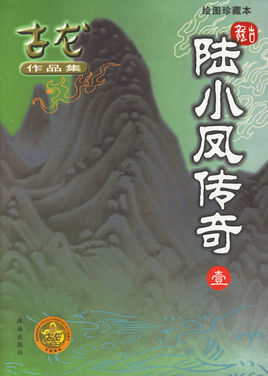
\includegraphics[width=.6\textwidth]{lxfbook.jpg}
\caption{陆小凤传奇\label{lxfbook}}
\end{figure}

\section{灵犀一指要诀}
灵犀一指是一种以柔制刚的武功,一般人很难领悟其中的精妙之处,因此很难学会。\cite{lxf:a}\citen{lxf:b}
实际上,它的要诀就是将内力汇聚在手指经脉之内,提高内力的密度,然后在瞬间释放出来,以致达到将敌人兵器折断的力道。
如表\ref{lxfinsight}所示。
\begin{table}
\centering
\caption{灵犀一指的要诀\label{lxfinsight}}
\begin{tabular}{|c||c|}
\hline
步骤 & 操作\\
\hline\hline
1 &  气聚丹田\\
\hline
2 & 将丹田之气注入手指经脉\\
\hline
3 & 瞬间释放\\
\hline
4 & 将敌人制服\\
\hline
\end{tabular}
\end{table}

也可用算法表示,如算法\ref{algoinsight}所示。

\begin{algorithm}
\caption{\label{algoinsight}灵犀一指要诀}
\begin{algorithmic}[1]
\STATE 气聚丹田。
\STATE 将丹田之气注入手指经脉。
\STATE 瞬间释放。
\STATE 将敌人制服。
\end{algorithmic}
\end{algorithm}

也可用数学公式表示,如式\ref{mc2}所示。
\begin{equation}
E=mc^2
\label{mc2}
\end{equation}

\section{本章小结}
本章介绍了灵犀一指的要诀部分。




\chapter{全文总结}
本文介绍了灵犀一指的起源,重要性和其中的要诀。
本章对全文工作进行了回顾和总结。

\acknowledgement
感谢每一个给予帮助的人。

\thesisbib{seuthesix}


\appendix

\chapter{欧几里得第二定理的证明}
\newtheorem{theorem}{定理}
\begin{theorem}
欧几里得第二定理(素数有无穷多个)\\
证明:用反证法。假设素数有有限个($N$个),记为$p_1,p_2,\dots,p_N$。则我们构造一个新的数,
\[
n=p_1p_2\dots p_N+1.
\]
由于$p_i,i=1,2,\dots,N$为素数,则一定不为$1$。于是对于任意的$p_i,i=1,2,\dots, N$,有
\[
p_i\not|n
\]
这表明,要么$n$本身为素数,要么$n$为合数,但是存在$p_1,p_2,\dots,p_N$之外的其他素数能够将$n$进行素因子分解。
不管哪种情况,都表明存在更多的素数。定理得证。\qed
\end{theorem}

\chapter{$\sqrt{2}$是无理数的证明}
\begin{theorem}
$\sqrt{2}$是无理数。\\
证明:用反证法。假设$\sqrt{2}$是有理数,则可表示为两个整数的商,即$\exists p,q, q\ne0$
\[
\sqrt{2}=\frac{p}{q}
\]
不失一般性,我们假设$p,q$是既约的,即$\gcd(p,q)=1$。对上式两边平方可得\\
\begin{align*}
2& =\frac{p^2}{q^2}\\
p^2&=2q^2.
\end{align*}
表明$p^2$为偶数,因此$p$为偶数,记$p=2m$。则
\begin{align*}
p^2&=4m^2=2q^2\\
q^2&=2m^2.
\end{align*}
表明$q$也为偶数,因此它们有公共因子$2$。这与它们既约的假设矛盾。定理得证。\qed
\end{theorem}

\resume{作者攻读硕士学位期间的研究成果}
\begin{flushleft}
{\bfseries \large 发表的论文}\\ \relax
[1] 第一作者,“灵犀一指:理论与应用”, 武侠学报,
2015年5月。\\
\end{flushleft}


\end{document}